%
% CAP�TULO: PUNTEROS
%

\chapter{Punteros}

%%
%% INTRODUCCION (ferda)
%%

%
% CAP�TULO: INTRODUCCI�N
%
\newpage
\ \
\newpage
\chapter{Introducci�n}
\section{Un poco de historia...}

El lenguaje de programaci�n C fue ideado e implementado por Dennis
Ritchie en 1972 en un DEC PDP-11\footnote{Un ordenador ``prehist�rico", enorme, con cintas, 
similar a los que salen en las pel�culas} usando UNIX como sistema operativo. Inicialmente, 
el est�ndar de C fue realmente la versi�n proporcionada por la 
implementaci�n de la versi�n V del sistema operativo UNIX. Su r�pida
expansi�n lleva a la aparici�n de varias variantes y problemas de
compatibilidad, por lo que en verano del 1983 se estableci� un comit�
para crear el est�ndar \textsc{ANSI}\footnote{Instituto Nacional de Est�ndares
Americano (American National Standards Institute)} para C. En 1989 se adopt� finalmente el est�ndar y poco despu�s
aparecieron los primeros compiladores conformes a este est�ndar. En 1995 se adopt� la 1� enmienda
con algunos cambios de la biblioteca de funciones, y fue la base para
desarrollar C++. Finalmente, en 1999 se adopt� el est�ndar C99 con
algunas mejoras e ideas prestadas de C++. Actualmente cohexisten las
dos versiones, mientras los programas migran a C99.

\section{Caracter�sticas}

\begin{itemize}
\item C es un lenguaje estructurado de nivel medio, ni de bajo
  nivel como ensamblador, ni de alto nivel como Ada o 
  Haskell. Esto permite una mayor flexibilidad y potencia, a cambio de
  menor abstracci�n.

\item No se trata de un lenguaje fuertemente tipado, lo que significa
  que se permite casi cualquier conversi�n de tipos. No es necesario que
  los tipos sean exactamente iguales para poder hacer conversiones,
  basta con que sean parecidos.

\item No lleva a cabo comprobaci�n de errores en tiempo de ejecuci�n,
  por ejemplo no se comprueba que no se sobrepasen los l�mites de los
  \textit{arrays}\footnote{Agrupaci�n de elementos de un mismo tipo de forma consecutiva  en memoria .
  Volveremos
  sobre los \textit{arrays} m�s tarde}. El programador es el �nico responsable de llevar a cabo esas
  comprobaciones.

\item Tiene un reducido numero de palabras clave, unas 32 en C89 y 37
  en C99. 
 
\item C dispone de una \emph{biblioteca est�ndar}
  que contiene numerosas funciones y que siempre est� disponible, adem�s de las extensiones que proporcione cada compilador o entorno
  de desarrollo.
\end{itemize} 

En resumen, es un lenguaje muy flexible, muy potente, muy popular,
pero que no protege al programador de sus errores.

\section{C frente a C++}

%Al principio es habitual no entender bien la diferencia entre C y C++,
%este �ltimo es un lenguaje para la programaci�n orientada a objetos
%que toma como base el lenguaje C. Se puede ver al C++ como una
%extensi�n de C para programaci�n orientada a objetos. \\

%En general, se puede utilizar un compilador de C++ para compilar un
%programa escrito en C, de hecho la mayor�a de los compiladores son
%para C/C++ indistintamente.

%----------------------------

No podemos hablar de C sin mencionar a C++, dado que es habitual no tener muy claro cuales 
son sus diferencias. En pocas palabras, C++ es un lenguaje para programaci�n orientada a objetos 
que toma como base el lenguaje C. La programaci�n orientada a objetos es otra filosof�a 
de programaci�n distinta a la de C (programaci�n estructurada)\footnote{ La programaci�n orientada a
objetos queda fuera del �mbito de este texto, para mas informaci�n se puede consultar cualquier libro de C++ } 
aunque con C++ es posible (aunque no especialmente recomendable) mezclar ambos estilos de programaci�n. 
En t�rminos generales, podemos ver a C++ como una extensi�n de C. Sin embargo, como se defini� 
a partir del est�ndar de C de 1989, y han evolucionado por separado, 
hay peque�as divergencias entre ellos.\\

Por lo general, se puede utilizar un compilador de C++ para compilar un 
programa escrito en C, inversamente la gran mayor�a de los programas 
escritos en C son v�lidos en C++. De hecho actualmente la mayor�a de los 
compiladores admiten tanto c�digo en C como en C++. 




%%
%% SINTAXIS (ferda)
%%

%% SECCI�N: SINTAXIS DE PUNTEROS

\section{Sint�xis de punteros}

\subsection{Declaraci�n de punteros}

Ante todo, \emph{un puntero es una variable}. Al dedicar un inter�s
especial en los punteros, puede dar la impresi�n de que son elementos
separados de las variables. No es as�. Son variables, y como veremos,
podemos asignarles nuevos valores, e incluso realizar algunas
operaciones aritm�ticas �tiles con ellos.\\

\emph{Una variable de tipo puntero est� �ntimamente ligada con el tipo
  al que apunta}. Por ello, en la declaraci�n, escribimos el nombre
  del tipo al que apuntar� nuestro puntero, seguido de asterisco, y por
  �ltimo, el nombre del puntero. Ejemplo:

\begin{verbatim}
int *p_entero;
float *p_real;
char *caracter;
\end{verbatim}

Ser�n declaraciones de punteros que contendr�n la direcci�n de memoria
de un entero, un real y un car�cter\footnote{Como veremos, la
  declaraci�n char * es usada tambi�n para la declaraci�n de
  cadenas de caracteres} respectivamente.

\subsection{Punteros gen�ricos}

Un caso especial, es cuando queremos declarar un puntero ``gen�rico'',
esto es, queremos que el puntero no est� ligado a ningun tipo
concreto. �Qu� sentido tiene esto?, como se ha visto previamente, en C
podemos realizar un \textit{cast} (ver \ref{cast}) sobre una variable,
y forzar su conversi�n a otro tipo. De esta manera, por ejemplo,
podr�amos declarar un puntero gen�rico, apuntar a una zona de memoria,
y realizar un cast sobre el puntero gen�rico.
\nota{La �nica diferencia existente entre un puntero
gen�rico, y un puntero ligado a un tipo de datos concreto, se produce
en las operaciones de aritm�tica de punteros (ver
\ref{punteros_aritmetica}).} 

Para declarar un puntero de tipo gen�rico, utilizamos:

\begin{verbatim}
void * pointer;
\end{verbatim}

Como veremos, muchas funciones de biblioteca de POSIX manejan punteros
gen�ricos en sus argumentos.

\subsection{Los operadores de contenido ``\texttt{*}'' y de indirecci�n
  ``\texttt{\&}''} 

\label{operadores_punteros}

El operador de indirecci�n \texttt{\&} se utiliza para referirse a la
direcci�n de una variable, as� el c�digo siguiente:

\begin{verbatim}
/* Reservamos 4 bytes para almacenar una direcci�n de memoria */
int *p_entero;

/* Reservamos 4 bytes para almacenar un entero */
int entero;

/* Escribimos en la variable p_entero la direcci�n de entero */
p_entero = &entero;
\end{verbatim}

Es totalmente correcto ya que, aunque la variable \texttt{entero} no
tenga ning�n valor asignado todav�a, lo que estamos haciendo es
escribir en la variable \texttt{p\_entero} la direcci�n de memoria
donde se almacena la variable \texttt{entero}.\\

\begin{figure}[H]
\begin{centering}
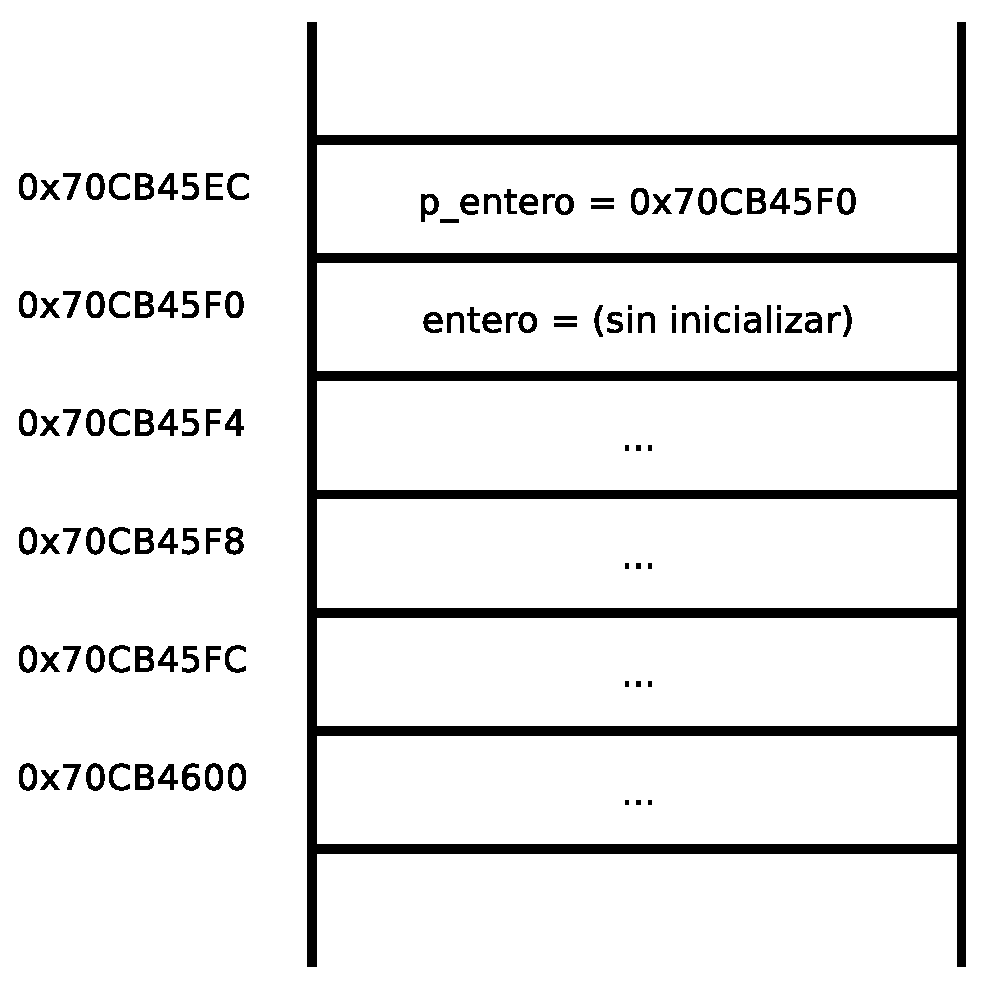
\includegraphics[width=80mm]{punteros/images/init_punteros.eps}
\caption{Inicializando punteros}
\end{centering}
\end{figure}

El operador \texttt{*} se utilizar para manejar la direcci�n a la que
apunta un puntero. Podr�amos llamarlo el operador de
\textit{acceso}. Tanto el operador de acceso, como el de indirecci�n,
funcionan en \textbf{notaci�n prefija}. Veamos un ejemplo que combina
ambos operadores:

\begin{verbatim}
1 int *p_entero;
2 int entero1, entero2;
3 entero1 = 2;
4 entero2 = 5;
5 p_entero = &entero1;
6 entero1 = *p_entero + entero2;
\end{verbatim}

Del mismo modo podemos asignar un valor a la variable a la que apunta
el puntero, de la forma:

\begin{verbatim}
1 int *p_entero;
2 int entero1, entero2;
3 entero1 = 2;
4 entero2 = 5;
5 p_entero = &entero1;
6 *p_entero = entero1 + entero2;
\end{verbatim}

Este �ltimo c�digo ejecutar�a \textbf{exactamente} lo mismo que el
anterior. Debemos notar que no tendr�a sentido prescindir de la linea
5, puesto que estar�amos intentando introducir el valor
\texttt{entero1 + entero2} en una direcci�n de memoria que no
conocemos, puesto que no le habriamos dado valor a \texttt{p\_entero}
(ver \ref{punteros_roma}).


%%
%% STRINGS (ana)
%%

%% SECCI�N: STRINGS  (autor: ana)

\section{Strings}
\label{strings}

Los arrays de caracteres se llaman \textbf{strings}. Funcionan
exactamente igual que cualquier otro array.  En los \textbf{strings}
no hace falta una variable que guarde el tama�o del array, puesto que
se marca el final del array con el car�cter ``\verb+\0+''.  La ventaja de los
\textbf{strings} es que podemos rellenar y consultar varios elementos
del array a la vez. En lugar de:

\begin{verbatim}
cadena[0] = 'h';
cadena[1] = 'o';
cadena[2] = 'l';
cadena[3] = 'a';
cadena[4] = '\0';
\end{verbatim}

Podremos hacer esto:

\begin{verbatim}
cadena = "hola";
/* cuando metemos un texto entre comillas dobles, al copiarlo al array
   el car�cter '\0' se incluye solo. */
print ("%s",cadena);
\end{verbatim}

Una serie de fallos comunes al trabajar con strings se exponen en
\ref{error_considerar_puntero}.\\

Existen funciones espec�ficas para trabajar con strings
(\verb+#include <string.h>+) para realizar ese tipo de
tareas. Recomendamos al lector que consulte la documentaci�n de
funciones como \textit{strlen, strcpy, strncpy, strdup, strcat}.


%%
%% ARITMETICA (jorge)
%%

%% SECCI�N: ARITMETICA DE PUNTEROS (autor: jorge)
\section{Aritm�tica de punteros}
\label{punteros_aritmetica}

Es posible realizar operaciones aritm�ticas sobre las variables de
tipo puntero para conseguir que apunten a una posici�n diferente.
Por ejemplo:

\begin{verbatim}

char cadena[5];
char *puntero;

puntero = &cadena[0]; /* puntero apunta a cadena[0] */
*puntero = 'h';       /* cadena[0] = 'h' */
*(puntero+1) = 'o';   /* cadena[1] = 'o' */
*(puntero+2) = 'l';   /* cadena[2] = 'l' */
*(puntero+3) = 'a';   /* cadena[3] = 'a' */
*(puntero+4) = '\0';  /* cadena[4] = '\0' */

\end{verbatim}

\begin{figure}[H]
\begin{centering}
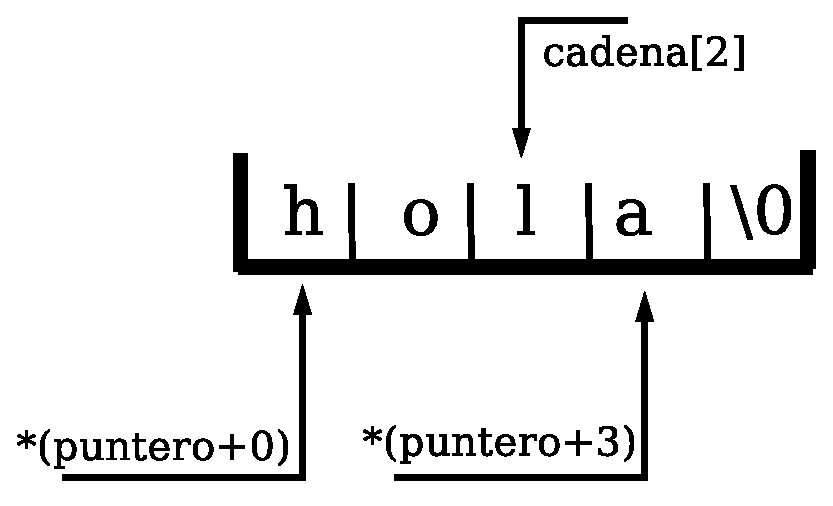
\includegraphics[width=70mm]{punteros/images/aritmetica0.eps}
\caption{Aritm�tica sobre un puntero}
\end{centering}
\end{figure}

\subsection{Contexto}

Se debe tener en cuenta que \verb-puntero+x- apuntar� a la direcci�n
de puntero sum�ndole \verb+x+ veces el espacio ocupado por un elemento
del tipo al que apunta, no el n�mero de bytes. 

\begin{figure}[H]
\begin{centering}
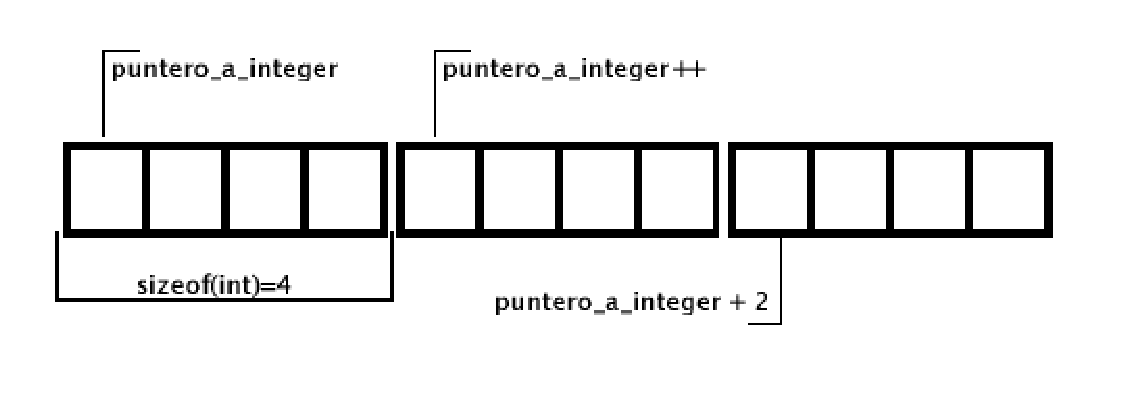
\includegraphics[width=130mm]{punteros/images/aritmetica1.eps}
\caption{Suma sobre un puntero a integer}
\end{centering}
\end{figure}

El programa mostrado a continuaci�n nos muestra la diferencia entre
considerar un puntero a integer y un puntero a char, en lo que se
refiere a la suma: 

\ejemplo{punteros/aritmetica/ejemplo_arit_punteros.c}

El resultado de ejecutar 
\footnote{Una vez m�s, recordamos que el tama�o de las variables en C
  es dependiente de la plataforma sobre la que compilemos/ejecutemos}
el c�digo anterior es:

\begin{verbatim}
Tama�o de int: 4
Tama�o de char: 1
Distancia entre punteros sucesivos a int : 4
Distancia entre punteros sucesivos a char: 1
\end{verbatim}

Queda clara la importancia entre declarar un puntero de un tipo o
otro. Ambos punteros del ejemplo ocupan lo mismo, ambos apuntan a
direcciones de memoria del sistema, pero cuando el compilador tiene
que generar c�digo para realizar operaciones aritm�ticas, lo hace de
manera distinta en funci�n del tipo de puntero.

\subsection{Tipos de operaciones}

Las operaciones soportadas sobre punteros son:

\begin{itemize}

\item Suma y resta de valores enteros ($+$,$-$,$++$ y $--$)
\item Comparaci�n y relaci�n ($<$,$>$,$<=$,$>=$,$==$ y $!=$)
\item Valor booleano (comparaci�n con NULL)

\end{itemize}

\subsection{Ejemplos de aritm�tica}

A continuaci�n mostramos un ejemplo de una funci�n que recibe dos
strings (ver \ref{strings}), y copia uno sobre otro. En la segunda
versi�n, las operaciones de aritm�tica de punteros se han agrupado,
para escribir menos c�digo. La finalidad de la segunda versi�n es
acostumbrar al lector a la complejidad de algunas operaciones en C
(funci�n \textit{copiar}).\\

Primera versi�n: 

\ejemplo{punteros/aritmetica/ejemplo_suma_punteros.c}

Segunda versi�n:

\ejemplo{punteros/aritmetica/ejemplo_suma_punteros_dificil.c}

Comentaremos la siguiente sentencia:

\begin{verbatim}
  while(*dest++ = *orig++); 
\end{verbatim}

Para entender la sentencia, la observaremos desde el punto de vista de la
precedencia entre operadores. En primer lugar, se ejecutar�an los
post-incrementos, pero su efecto s�lo tendr�a lugar al acabar la
sentencia (la expresi�n parentizada). Por tanto, lo siguiente en
ejecutarse ser�a el operador de acceso (``*''). Eso acceder�a a los
caracteres apuntados por \verb+dest+ y por \verb+orig+. Despu�s se ejecutar�a la
asignaci�n, (copia de un car�cter de la cadena). Como se vi� en
\ref{operador_asignacion}, la asignaci�n ``devuelve'' el valor
asignado, por lo que la expresi�n parentizada equivale al valor que se
asigna. Cuando se asigna el �ltimo car�cter de la cadena (\verb+\0+),
el valor de la expresi�n es falso (\verb+\0+ equivale a 0, esto es,
falso), y el  \verb+while+ saldr�a. Antes de terminar de procesar, se
incrementar�an ambos punteros (post-incrementos), haciendo que apunten
al siguiente car�cter de la cadena.

\consejo{Normalmente el uso de la aritm�tica de punteros se centra en
operaciones sencillas de incremento o decremento.  Operaciones m�s
complejas son potencialmente peligrosas, adem�s operaciones como la
multiplicaci�n o divisi�n de dos apuntadores no estan permitidas lo
cual es bastante l�gico debido a la m�nima utilidad pr�ctica de estos
operadores en punteros. A la hora de programar se debe recordar que
un mal uso de la aritm�tica de punteros puede dejar poco portable 
nuestro c�digo.}



%%
%% STRUCTS Y PUNTEROS (ferda)
%%

%% SECCI�N: ESTRUCTURAS Y PUNTEROS
\section{Estructuras y punteros}

\subsection{El operador ``\texttt{->}''}
\label{operador_puntero_structs}

En programas un poco m�s elaborados, usaremos a menudo los punteros
para apuntar a estructuras (\texttt{struct}). Nada nos impide
referirnos a los campos de la estructura a la que apunta el puntero de
la forma que hemos visto hasta ahora, es decir, llamando al campo que
deseemos del contenido del puntero dado. Con este ejemplo entenderemos
mejor a qu� nos referimos:

\begin{verbatim}
struct coordenada {
   int x, y;
} coord;
struct coordenada *p_coord;
p_coord = &coord;
(*p_coord).x = 4;
(*p_coord).y = 3;
\end{verbatim}

\begin{flushleft}
Aun as� esto puede resultar algo engorroso, por eso C nos da la
posibilidad de usar el operador \texttt{->} que nos facilita las
cosas:
\end{flushleft}

\begin{verbatim}
struct coordenada {
   int x, y;
} coord;
struct coordenada *p_coord;
p_coord = &coord;
p_coord->x = 4;
p_coord->y = 3;
\end{verbatim}

Los dos c�digos anteriores ejecutan lo mismo pero en el segundo
utilizamos el operador \texttt{->}, que nos hace el c�digo m�s
legible. 

\nota{Es un error frecuente utilizar el operador punto sobre un
puntero a estructura.}  
 

%%
%% MEMORIA DINAMICA (mustang)
%%

%% SECCI�N: MEMORIA DIN�MICA (autor: mustang)

\section{Memoria din�mica}

\label{mem_dinamica}

\subsection{�Qu� es la memoria din�mica?}

Supongamos que nuestro programa debe manipular estructuras de datos de
longitud desconocida. Un ejemplo simple podr�a ser el de un programa
que lee las l�neas de un archivo y las ordena. Por tanto, deberemos
leer un n�mero indeterminado de l�neas, y tras leer la �ltima,
ordenarlas. Una manera de manejar ese ``n�mero indeterminado'', ser�a
declarar una constante \verb+MAX_LINEAS+, darle un valor
vergonzosamente grande, y declarar un array de tama�o
\verb+MAX_LINEAS+. Esto, obviamente, es muy ineficiente (y
feo). Nuestro programa no s�lo quedar�a limitado por ese valor m�ximo,
sino que adem�s gastar�a esa enorme cantidad de memoria para procesar
hasta el m�s peque�o de los ficheros.\\

La soluci�n consiste en utilizar memoria din�mica. La memoria din�mica
es un espacio de almacenamiento que se solicita \textit{en tiempo de
ejecuci�n}\footnote{cuando el programa llega al punto en el que
necesita espacio para una l�nea m�s}. De esa manera, a medida que el
proceso va necesitando espacio para m�s l�neas, va solicitando m�s
memoria al sistema operativo para guardarlas. El medio para manejar la
memoria que otorga el sistema operativo, es el puntero, puesto que no
podemos saber \textit{en tiempo de compilaci�n}\footnote{es decir, al programar}
d�nde nos dar� huecos el sistema operativo (en la memoria de nuestro
PC). 

\subsection{El mapa de memoria en Unix}

Antes de profundizar en el manejo de memoria din�mica, vamos a dar una
breve visi�n del mapa de memoria en Unix, esto es, c�mo se organiza la
memoria de un proceso. Ante todo, esto es una simplificaci�n, para
poder situar mejor los punteros en su contexto.\\

De entre las varias regiones de memoria que existen, hay dos que nos
interesan al hablar de punteros (y sobre todo, al depurar): la pila y
el heap. 

\subsubsection{La pila}

En ingl�s, stack. Su contenido se estudia en profundidad en las
asignaturas de \textit{Laboratorio de Estructura de Computadores} y
\textit{Compiladores}. Aqu� solo diremos que cada vez que se realiza
una llamada a una funci�n, se introduce en la pila una estructura que
almacena los par�metros pasados a la funci�n, y las variables
declaradas dentro de ella. Cuando la funci�n retorna, dicha estructura
es destruida. 

\subsubsection{El heap}

Esta regi�n queda disponible para las solicitudes de memoria din�mica
al sistema operativo. Su crecimiento va ligado a la disminuci�n de la
pila, y viceversa. 

\begin{figure}[H]
\begin{centering}
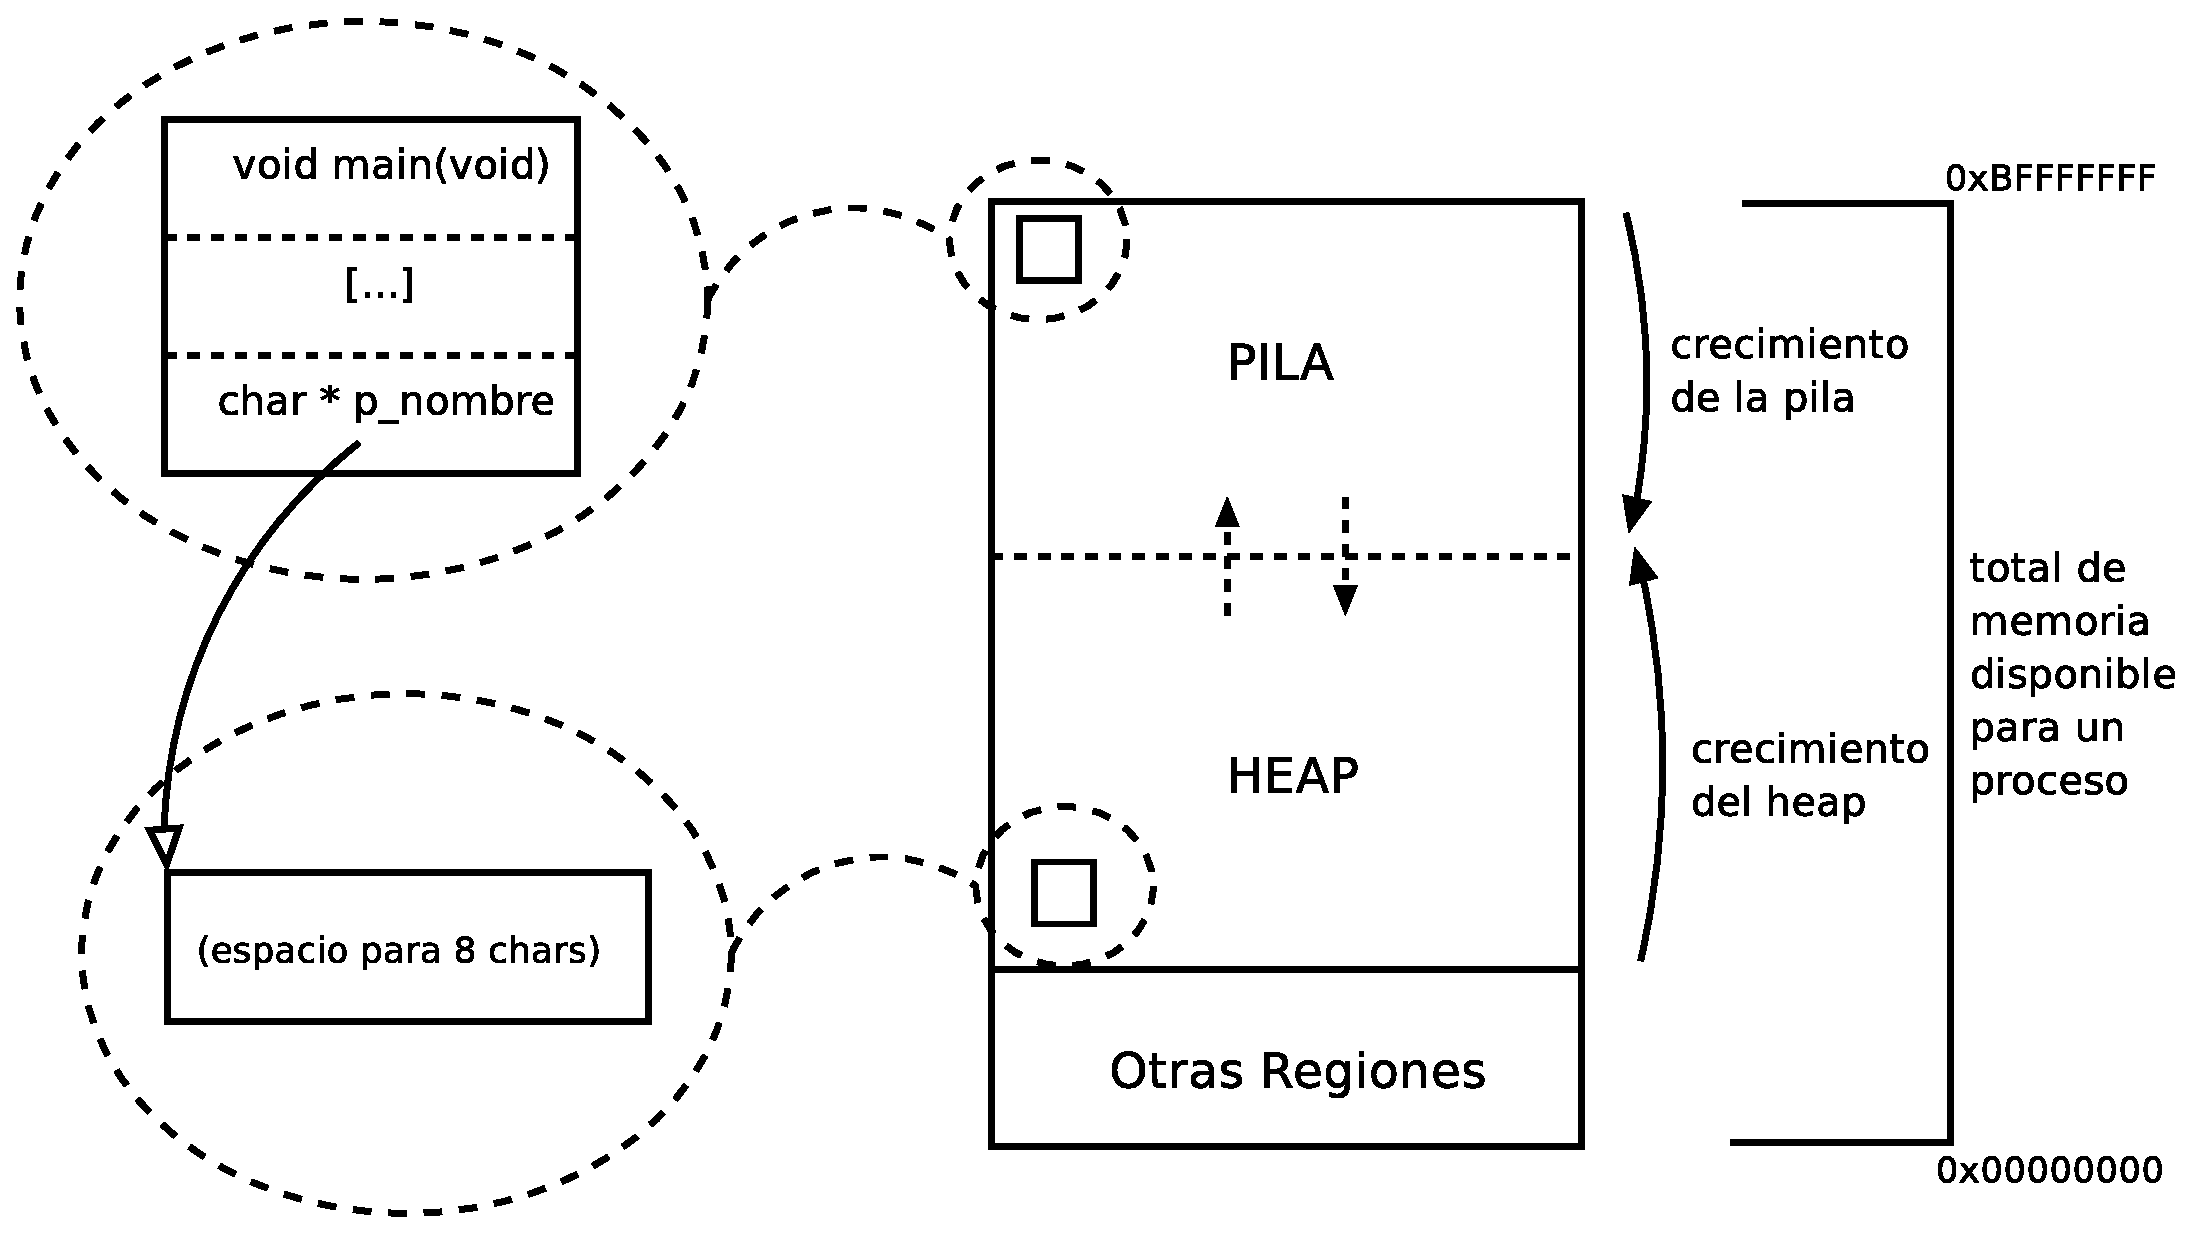
\includegraphics[width=145mm]{punteros/images/pila_heap.eps}
\caption{Visi�n general del mapa de memoria}
\end{centering}
\end{figure}

La figura anterior, muestra el resultado de solicitar al sistema
operativo espacio en memoria din�mica para 8 chars. Podemos quedarnos
con la idea de que las variables locales de una funci�n, y los
argumentos de la misma van en la pila, mientras que la memoria
din�mica va en el heap.

\subsection{Primitivas b�sicas}

Las primitivas b�sicas para el manejo de memoria din�mica son: 

\begin{itemize}
\item \verb+malloc+
\item \verb+realloc+
\item \verb+free+
\end{itemize}

\subsubsection{\texttt{malloc}}

Solicita memoria din�mica al sistema operativo. Su prototipo es:

\begin{verbatim}
void *malloc(size_t size);
\end{verbatim}

Devuelve un puntero tipo void, que apunta a la zona solicitada, o
NULL, en caso de no poderse cumplir la solicitud (probablemente por
falta de memoria libre). El tipo \verb+size_t+, tiene conversi�n
directa desde los \verb+int+.\\

Por ejemplo, si quisi�ramos solicitar memoria din�mica para almacenar
8 chars:

\begin{verbatim} 
char *p_char;
p_char = malloc(8*sizeof(char));
\end{verbatim}

No obstante, el autor prefiere especificar a mano los cast (ver
\ref{cast}) que se deben realizar para que encajen los argumentos:

\begin{verbatim} 
char *p_char;
p_char = (char *) malloc( (size_t) 8*sizeof(char));
\end{verbatim}

\nota{La zona de memoria devuelta por \texttt{malloc} no se inicializa a
  ning�n valor concreto.}

\subsubsection{\texttt{realloc}}

Cambia el tama�o de una zona de memoria din�mica, pedida al sistema
operativo previamente mediante la orden \verb+malloc+. Su prototipo es: 

\begin{verbatim}
void *realloc(void *ptr, size_t size);
\end{verbatim}

\begin{flushleft}
Un ejemplo de uso de \verb+realloc+:
\end{flushleft}

\begin{verbatim}
char *p_char;
int size;

size = 8 * sizeof(char);

/* pedimos memoria en p_char */
p_char = (char *) malloc( (size_t) size); 

[.....]

/* necesitamos m�s memoria en p_char */
size *= 2;
p_char = (char *) realloc(p_char, (size_t) size);
\end{verbatim}

\begin{flushleft}
Un ejemplo habitual de uso de \texttt{realloc} est� en
\ref{ejemplo_realloc_duro}. 
\end{flushleft}

\nota{\texttt{realloc} puede devolvernos la zona de memoria solicitada
  en otra posici�n. Esto es, independientemente de encargarse de
  reservar el nuevo espacio solicitado, el puntero que retorna \texttt{realloc}
  puede ser distinto al devuelto originalmente por \texttt{malloc}. Aun as�,
  \texttt{realloc} se encarga de que el contenido apuntado por el puntero sea
  el mismo. Dicho de otra manera, si pedimos memoria para x
  caracteres, y luego hacemos \texttt{realloc} sobre esa zona pidiendo x+n
  caracteres, \texttt{realloc} se encargar� de que los x primeros caracteres de
  la zona devuelta (sea la misma zona pero m�s grande, o sea otra zona
  distinta) sean id�nticos. Como es habitual, si solicitamos m�s
  espacio, ese espacio extra no ser� inicializado.}

\subsubsection{\texttt{free}}

Libera una zona de memoria din�mica, solicitada previamente mediante
\verb+malloc+. Su prototipo es: 

\begin{verbatim}
void free(void *ptr);
\end{verbatim}

\begin{flushleft}
Un ejemplo de uso de \texttt{free}:
\end{flushleft}

\begin{verbatim}


char *p_char;

/* pedimos memoria en p_char */
p_char = (char *) malloc( (size_t) 8*sizeof(char)); 

[...]

free(p_char);
\end{verbatim}

\nota{Liberar una zona de memoria una segunda vez es
  ilegal (ver \ref{error_doble_liberacion}).}

\nota{Es habitual al empezar a manejar memoria din�mica, dejar la
  tarea de liberar la memoria solicitada para el final. Esto es una
  mala pol�tica de trabajo. Por cada \texttt{malloc} que utilizamos, debemos
  pensar donde se va a hacer su \texttt{free}, y colocar ambos en el c�digo. En
  cuanto los programos crecen, es habitual olvidarse de liberar
  memoria, y el consumo de nuestros programas pueden crecer de manera
  desorbitada.}

\subsubsection{strdup}

Es una primitiva incluida en \textit{string.h}. La hemos incluido en
el manual, porque se usa frecuentemente, aunque al igual que strdup,
hay muchas llamadas al sistema similares (piden memoria din�mica por
nosotros). Su prototipo es:

\begin{verbatim}
  char *strdup(const char *s);
\end{verbatim}

Es una funci�n bastante c�moda, le suministramos un puntero a un
string, y nos devuelve un puntero a una zona de memoria din�mica, que
es una copia de la cadena que le hemos pasado. Dicho de otra manera,
strdup equivale a hacer un \texttt{malloc} de la longitud de la cadena
argumento, y a copiarla sobre la zona devuelta. Un ejemplo de uso ser�a:

\begin{verbatim}
char * pointer;
char * data = "Hello world\n";

pointer = strdup(data);

printf("%s", pointer);

free(pointer);
\end{verbatim}
%"

Este caso es un candidato ideal para mostrar un error frecuente al
trabajar con strings y punteros (ver
\ref{error_confundir_strings_punteros}).


%%
%% ARRAYS Y PUNTEROS (ana)
%%

%% SECCI�N: ARRAYS Y PUNTEROS  (autor: ana)
\section{Arrays y punteros}
\label{arrays_punteros}

\begin{flushleft}
Hasta ahora para nosotros un array era un conjunto ordenado de
elementos del mismo tipo.
\end{flushleft}

\subsection{Repaso}

\begin{flushleft}
La sintaxis en C para declarar un array es:
\end{flushleft}

\begin{verbatim}
tipo_elementos nombre_array[numero_elementos];
\end{verbatim}

\begin{flushleft}
La sintaxis para acceder a sus elementos es:
\end{flushleft}

\begin{verbatim}
nombre_array[indice]
\end{verbatim}

\begin{flushleft}
Ejemplo: un array de cinco elementos que contenga n�meros primos ser�a as�:
\end{flushleft}

\begin{verbatim}
int numeros_primos[5];

numeros_primos[0] = 2;
numeros_primos[1] = 3;
numeros_primos[2] = 5;
numeros_primos[3] = 7;
numeros_primos[4] = 11;
\end{verbatim}

\subsection{Introducci�n}

Ahora vamos a ver qu� es para el compilador un array, y as�
aprenderemos a usarlos de manera m�s eficiente. Un array es un
conjunto de elementos del mismo tipo. Para que sea conjunto
``ordenado'', lo que el compilador hace es juntar todos los elementos
en la misma zona de memoria. Almacena la direcci�n inicial en nuestra
variable para saber d�nde est� el primer elemento, que corresponder�a
al �ndice ``0''. A partir de ah�, al incrementar la direcci�n de
memoria en el tama�o de los elementos, va accediento a array[1],
array[2], etc.

\begin{figure}[H]
\begin{centering}
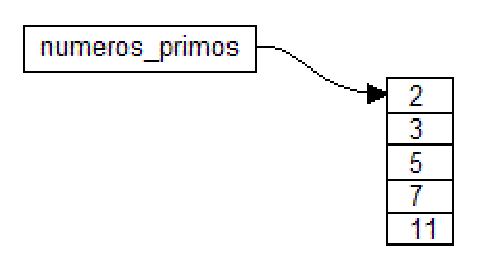
\includegraphics[width=65mm]{punteros/images/arrays_1.eps}
\caption{Un array de n�meros primos}
\end{centering}
\end{figure}

\begin{figure}[H]
\begin{centering}
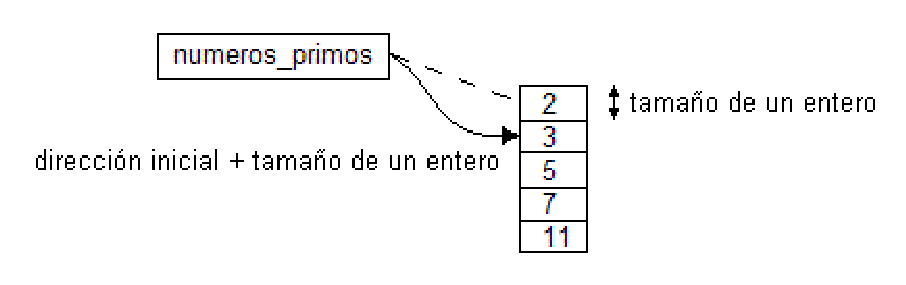
\includegraphics[width=115mm]{punteros/images/arrays_2.eps}
\caption{Avanzando sobre un array}
\end{centering}
\end{figure}

As� podemos deducir la siguiente f�rmula: 
\textit{direcci�n\_elemento$=$direcci�n\_inicial$+($�ndice$*$tama�o\_elementos$)$}.\\

Esta f�rmula es la que aplica el compilador para calcular la direcci�n
del elemento al que nos referimos al hacer un acceso al array del tipo
\textit{array[indice]}, como por ejemplo \textit{numeros\_primos[3]}.
Claramente, se dibuja la idea del puntero en el concepto de
array:\\

\definicion{Variable tipo array}{Un puntero al primer elemento del
array.}

�Cu�l es la ventaja de trabajar de punteros, con los posibles
problemas que eso trae, en vez de con arrays sin m�s?  La respuesta
surge enseguida: un array tiene un tama�o fijo desde su
declaraci�n. Sin embargo, trabajando con punteros, nuestro array podr�
tener el tama�o que nosotros queramos durante el programa, y podemos
incluso variarlo en funci�n de otros datos del programa.\\

Por supuesto, esta ventaja tiene un precio (aunque muy bajo) que no
debemos olvidar. Debemos apuntar en alg�n sitio (variable, constante)
cu�nto espacio hemos pedido y en otro cu�nto de ese espacio hemos
aprovechado. Como al programar no conoceremos el espacio aprovechado
del array, deberemos hacer una de estas dos cosas:

\begin{itemize}
\item apuntar en otra variable el tama�o ocupado del array.  
\item hacer que el �ltimo elemento del array sea diferente, un dato
  que no nos puedan introducir, por ejemplo, un n�mero negativo o una letra cuando hablamos
  de n�meros de tel�fono. 
\end{itemize}

\begin{figure}[H]
\begin{centering}
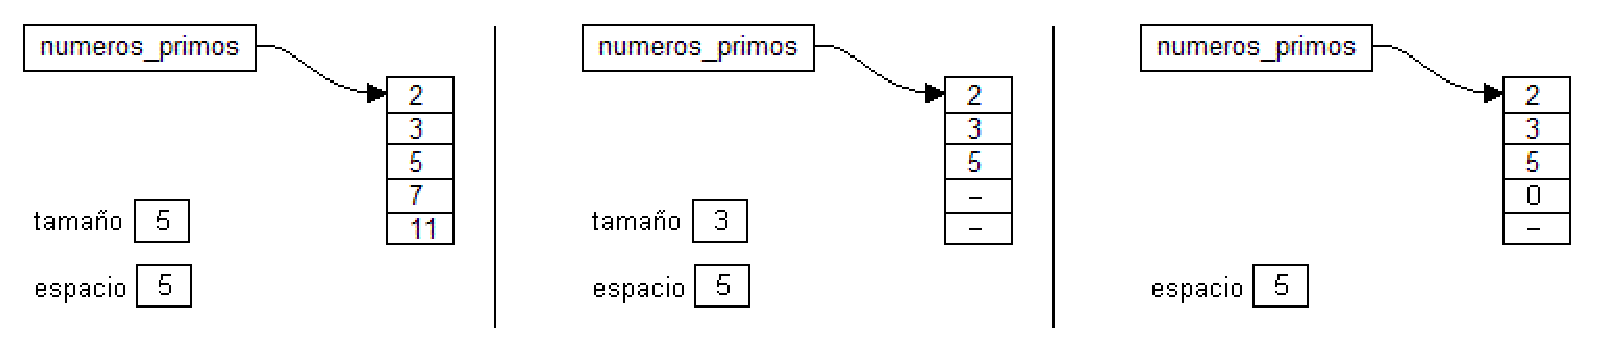
\includegraphics[width=170mm]{punteros/images/arrays_3.eps}
\caption{M�s sobre arrays}
\end{centering}
\end{figure}

\paragraph{Ejemplo}
Queremos que el usuario introduzca varios n�meros de tel�fono y los
vamos a almacenar en el array \textit{telefonos}. No sabemos cu�ntos
n�meros va a introducir el usuario. Si lo tuvi�ramos que implementar
con un array definido desde su
declaraci�n, tendr�amos que poner un tope a los n�meros de tel�fono
que se pueden introducir, por ejemplo 10:

\begin{verbatim}
int i;
int telefonos[10];

i=0;
while (usuario_introduce && (i<10))
{
  telefonos[i] = numero_introducido;
  i++;
}
numeros_introducidos = i;
\end{verbatim}

Sin embargo, trabajando con punteros podemos preguntar al usuario
cu�ntos n�meros quiere introducir:

\begin{verbatim}
int i, tamano;
int *telefonos; // o bien: int telefonos[]

telefonos = NULL;
/* es muy recomendable inicializar el valor de un puntero a NULL.
 * As�, si se nos olvida pedir memoria para �l, el programa fallar� siempre.
 * Por el contrario, si no lo inicializamos, el programa fallar� 
 * algunas veces s� y otras no. */

tamano = preguntar_tamano();
telefonos = malloc (tamano);

for (i=0;i<tamano;i++)
  telefonos[i] = numero_introducido;
\end{verbatim}

O tambi�n variar el tama�o del array de forma din�mica:

\begin{verbatim}

int i, tamano, nuevo_tamano;
int *telefonos; // o bien: int telefonos[]

telefonos = NULL;
i=0;
while (usuario_introduce)
{
  nuevo_tamano = sizeof (int) * (i+1);
  telefonos = realloc (telefonos,nuevo_tamano);
  telefonos[i] = numero_introducido;
  i++;
}
tamano=i;
\end{verbatim}

\nota{Si el tama�o del array es ``X'', los �ndices (que empiezan por cero) ir�n de ``0'' a ``X-1''.}



%%
%% INDIRECCIONES MULTIPLES (luisc)
%%

%% SECCI�N: INDIRECCIONES M�LTIPLES
\section{Indirecciones m�ltiples}

Una herramienta muy �til que proporciona C en su manejo de punteros
son las indirecciones m�ltiples, es decir, punteros que apuntan a
punteros. Las indirecciones pueden ser dobles, triples, cuadruples \dots.

\subsection{Declaraci�n}

Ejemplo:

\begin{verbatim}
char **ind_doble;
char ***ind_triple;
\end{verbatim}

La primera declaraci�n declarar�a un puntero de indirecci�n doble de
tipo char (l�ase: puntero que apunta a puntero), mientras que la
segunda declarar�a un puntero de indirecci�n triple a char (puntero
que apunta un puntero que apunta a otro puntero [es decir, un
l�o]). Usar m�s de indirecci�n triple es abiertamente desaconsejable.

\begin{figure}[H]
\begin{centering}
\includegraphics[width=110mm]{punteros/images/ind_doble.eps}
\caption{Indirecci�n doble}
\end{centering}
\end{figure}

\begin{figure}[H]
\begin{centering}
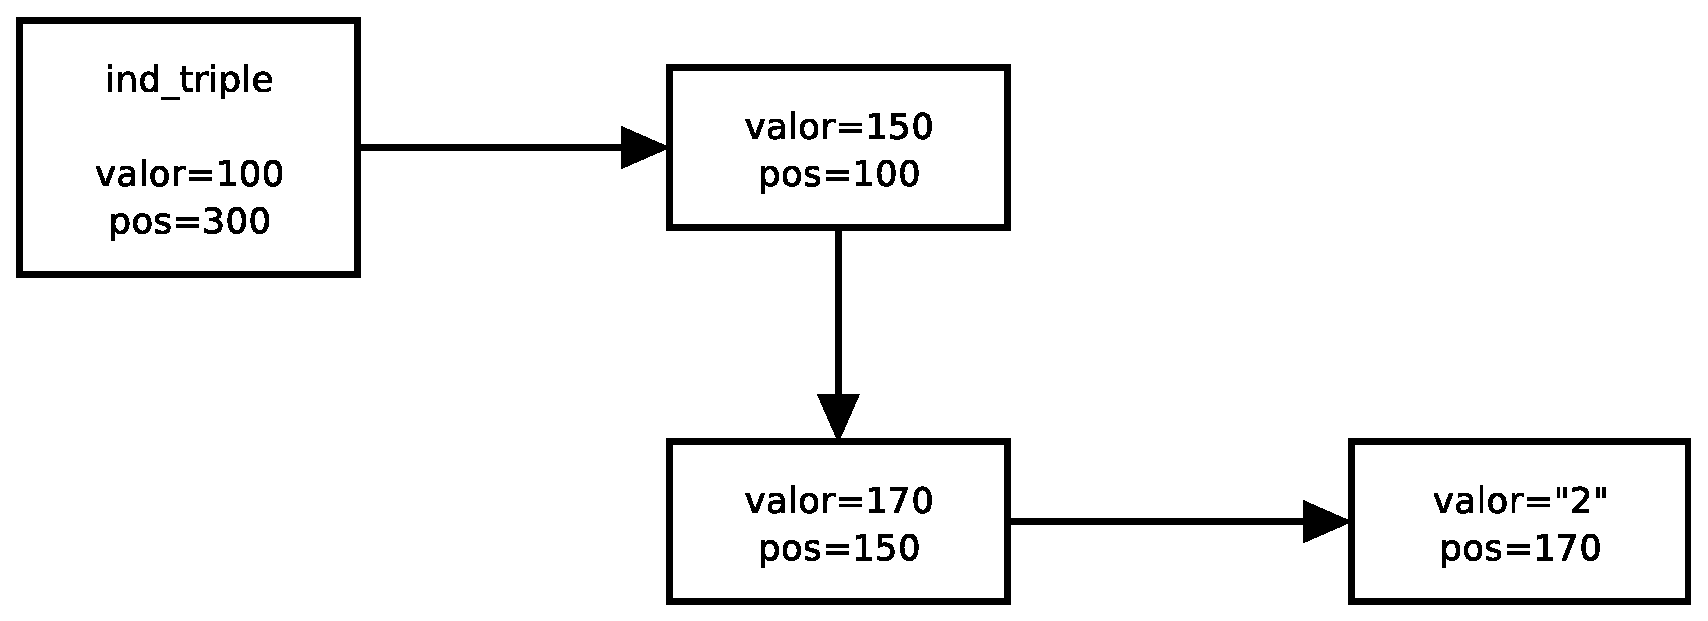
\includegraphics[width=110mm]{punteros/images/ind_triple.eps}
\caption{Indirecci�n triple}
\end{centering}
\end{figure}

\subsection{Utilizaci�n}

\begin{verbatim}
char **ind_doble;
char *puntero_normal;

/* Este acceso nos dar�a la direcci�n de la primera indirecci�n */

puntero_normal = *ind_doble;

/* Estos dos accesos ser�an equivalentes (despues de la asignaci�n de
 * arriba) */
 
*puntero_normal = 'A';
**ind_doble = 'A';
\end{verbatim}

Esto es as� porque \verb+*ind_doble+, es un puntero a char, es decir,
como regla cada \verb+*+ que pongamos en un puntero con indirecci�n
m�ltiple quitamos un nivel de indirecci�n.\\

Una vez m�s, recordar la dualidad entre �ndices de array y
punteros. Por ejemplo, cuando tratamos con un puntero de doble
indirecci�n, como puede ser \verb+char **data+, las expresiones
\begin{itemize}
\item\verb-data[1][2]- y 
\item \verb-*(*(data+1)+2)- 
\end{itemize}
son equivalentes.

\paragraph{Ejemplo}

\begin{itemize}
\item \verb+*ind_doble+ ser�a un puntero simple (de los vistos
  anteriormente).
\item \verb+**ind_doble+ ser�a el valor apuntado, es decir el
  car�cter de los ejemplos anteriores.
\item \verb+*ind_triple+ ser�a un puntero de indirecci�n doble.
\end{itemize}

\subsection{Ejemplos de uso}

Uno de los usos de punteros de indirecci�n m�ltiple, es, por ejemplo,
leer un texto completo y almacenarlo por l�neas.

\begin{verbatim}
char **texto;
\end{verbatim}

Cada \verb+*texto+ ser�a una l�nea, y cada \verb+**texto+ una letra de
la l�nea seleccionada. Ve�moslo con un programa:

\ejemplo{punteros/multiples/ejemplo_punteros_multiples.c}

\label{ejemplo_realloc_duro}
El siguiente ejemplo es especialmente interesante, combina el uso de
\verb-malloc- y \verb-realloc- con indirecciones m�ltiples. El programa utiliza un
doble puntero, sobre el que ejecuta un \verb-malloc-, y posteriormente, un
\verb-realloc- por cada nueva l�nea que vayamos leyendo. En cada nuevo
espacio que devuelve \verb-realloc-, se ejecuta un \verb-malloc- para almacenar una
nueva l�nea de texto.

\ejemplo{punteros/multiples/multiples_realloc.c}

Debemos tener en cuenta que el orden de los \verb-free- es importante:
primero liberamos cada uno de los \verb-malloc- que se ejecutaron dentro del
bucle (zonas sueltas de memoria, que almacenan una l�nea cada una). Al
final, liberamos el doble puntero, sobre el que hemos ejecutado un
\verb-malloc-, y varios \verb-realloc-. Si hici�ramos la liberaci�n al rev�s,
estar�amos pas�ndole como argumento a \verb-free-, punteros situados en una
zona de memoria que ha sido liberada (ya no es nuestra). El
comportamiento ser�a impredecible. \\

Como se vi� en la secci�n \ref{arrays_punteros}, es indiferente
acceder a un puntero m�ltiple usando la notaci�n de los arrays o el
operador de acceso junto con la aritm�tica de punteros:

\begin{verbatim}
double ** pointer;
double * p1;

p1 = (double *) malloc((size_t) 8 * sizeof(double));
pointer = &p1;  /* pointer apunta a p1 */

pointer[0][0]=3.141592;
pointer[0][1]=6.022E23;

printf("%g %g\n",pointer[0][0], pointer[0][1]);
printf("%g %g\n",**pointer, *(*pointer+1));
\end{verbatim}

\subsection{Cadenas enlazadas}

Uno de los usos m�s utiles de punteros es la implementaci�n de las
cadenas enlazadas, que se estudian en la asignatura de
\textit{Estructura de Datos I}.\\

El tipo \verb+cadena_enlazada+ es un puntero a un nodo, consistente de
un puntero al siguiente nodo (una cadena\_enlazada en si misma) y un
dato de un tipo cualquiera.\\

La dificultad de implementar es qu� tipo declarar primero, nodo o
cadena\_enlazada. Para ello, usaremos una t�cnica conocida como
\textit{forward declaration}. La idea consiste en avisar al compilador
de que estamos declarando un tipo, que es un puntero a una estructura,
pero que dicha estructura a�n no la hemos declarado, la declararemos
despu�s. 

\begin{figure}[H]
\begin{centering}
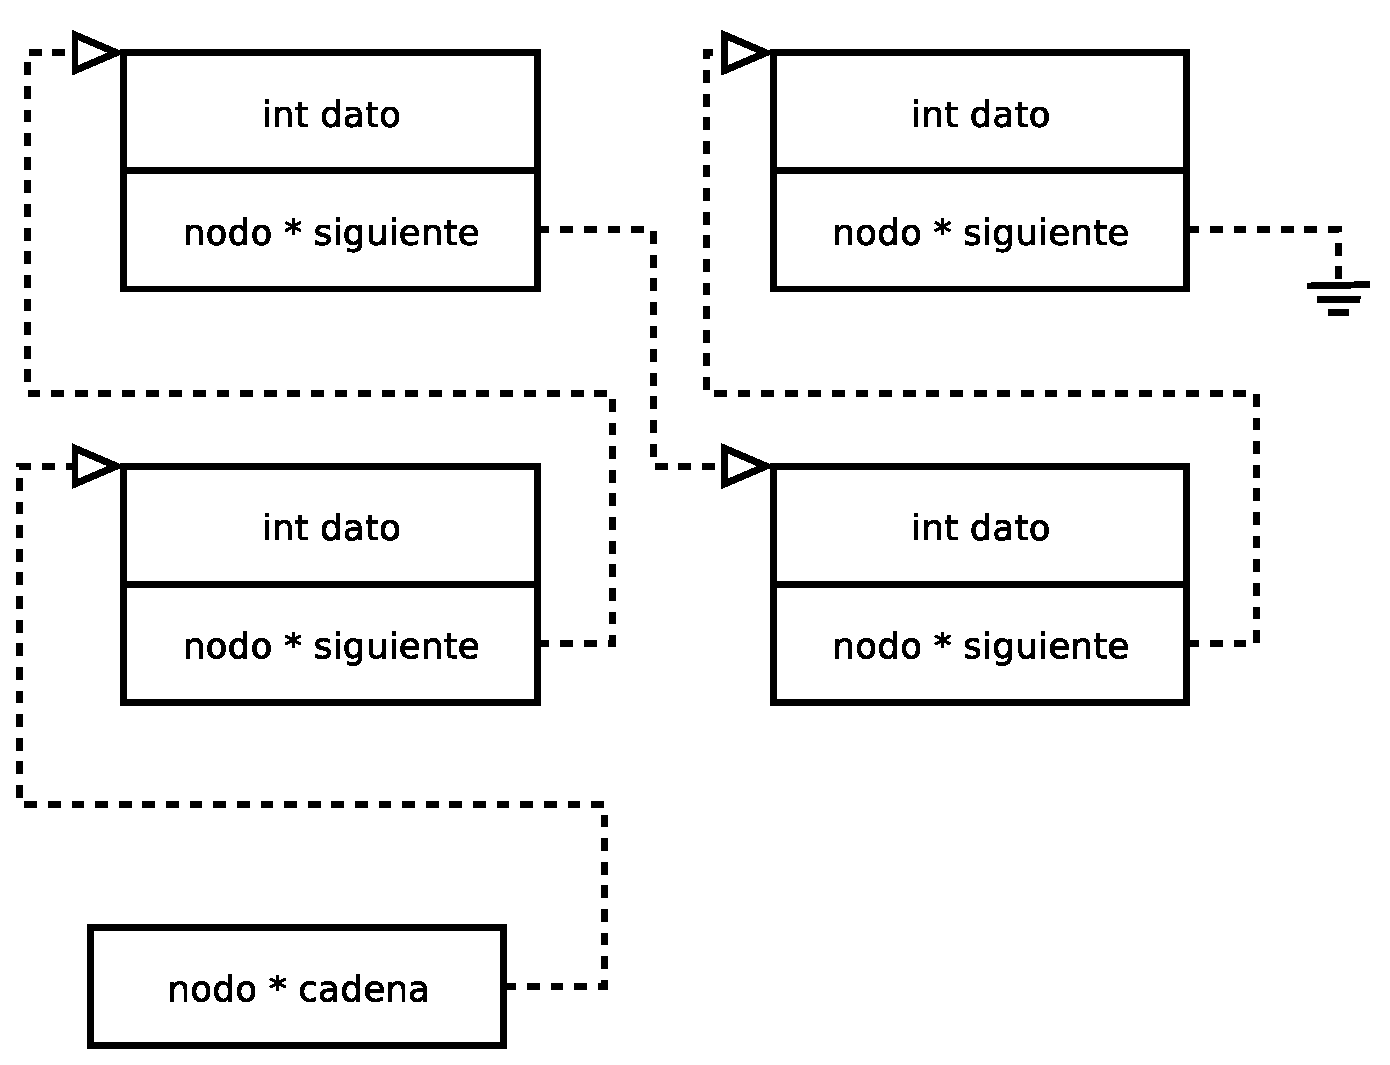
\includegraphics[width=100mm]{punteros/images/cadenas.eps}
\caption{Ejemplo de una cadena enlazada}
\end{centering}
\end{figure}

Una manera incorrecta de implementarlas ser�a:

\begin{verbatim}
typedef nodo * cadena_enlazada;

struct nodo{
  cadena_enlazada siguiente;
  int dato;
}
\end{verbatim}

debido a que el compilador no tiene definido el tipo \verb+nodo+ en el
momento de definir \verb+cadena_enlazada+. La forma correcta ser�a:

\begin{verbatim}
typedef struct nodo *cadena_enlazada;
        
struct nodo{
  cadena_enlazada siguiente;
  int dato;
};
\end{verbatim}

o tambi�n, si quisieramos realizar el \verb-typedef- sobre ambos tipos:

\begin{verbatim}
typedef struct nodo *cadena_enlazada;
        
typedef struct nodo{
  cadena_enlazada siguiente;
  int dato;
};
\end{verbatim}

Un ejemplo de uso de las cadenas enlazadas es:

\ejemplo{punteros/multiples/enl.c}



%%
%% PASO POR REFERENCIA vs PASO POR VALOR (cps)
%%

%% SECCI�N: PASO POR REFERENCIA vs PASO POR VALOR

\newpage

\section{Paso por referencia vs. paso por valor}

\label{valor_vs_referencia}

\subsection{�Qu� es el paso por referencia?}

A la hora de pasar una variable como argumento a una funci�n, el paso
por referencia consiste en entregar como argumento un puntero a la
variable, y no el contenido de la variable.

\subsection{�Para qu� necesito el paso por referencia?}

Si tratamos de modificar los valores de los argumentos de una funci�n, 
estos cambios no ser�n vistos desde fuera de la misma. Esto es debido
a que los argumentos de la funci�n son copias de las variables reales y
 son almacenadas como variables locales a dicha funci�n, desapareciendo 
por tanto al regresar a la llamante. Se incluye un ejemplo a continuaci�n:

\ejemplo{punteros/referencia_valor/no_mod_args.c}

Si compilamos y ejecutamos el c�digo anterior, obtenemos el 
siguiente resultado:
\begin{verbatim}
Variable var1 = 1
Variable var1 = 1
\end{verbatim}

Como era de esperar, no se ha modificado el valor de la variable \texttt{var1}
fuera de la funci�n.

Por esto, si queremos modificar el valor de un argumento en una funci�n,
debemos pasar este par�metro \textit{por referencia}, como se muestra
en el siguiente ejemplo:

\ejemplo{punteros/referencia_valor/mod_args.c}

Como se puede comprobar, la salida de este programa es correcta:
\begin{verbatim}
Variable var1 = 1
Variable var1 = 2
\end{verbatim}

Si en una funci�n quisi�ramos modificar un par�metro que fuera un puntero, 
ser�a necesario pasar como argumento la direcci�n del mismo, es decir, 
\textit{doble indirecci�n}. Y as� sucesivamente si el argumento fuera 
doble puntero, triple puntero, etc. \\

Tambi�n es muy aconsejable el paso por referencia en el caso en que una funci�n
reciba como argumento una gran estructura de datos (arrays, matrices, ...),
puesto que el paso por valor implicar�a una copia completa de la estructura
en el espacio de memoria de la funci�n.


%%
%% ERRORES CON PUNTEROS (cps)
%%

%% SECCI�N: ERRORES CON PUNTEROS

\section{Errores con punteros}

\subsection{Comparaci�n de punteros a cadenas}
\label{error_confundir_strings_punteros}

Un error que ocurre frecuentemente al empezar a programar en C 
es intentar comparar dos cadenas de caracteres mediante sus punteros.
Ve�moslo en el siguiente ejemplo:

\ejemplo{punteros/errores/strings.c}

En la ejecuci�n de este programa, tendr�amos la siguiente asignaci�n
de memoria:

\begin{figure}[H]
  \begin{center}
    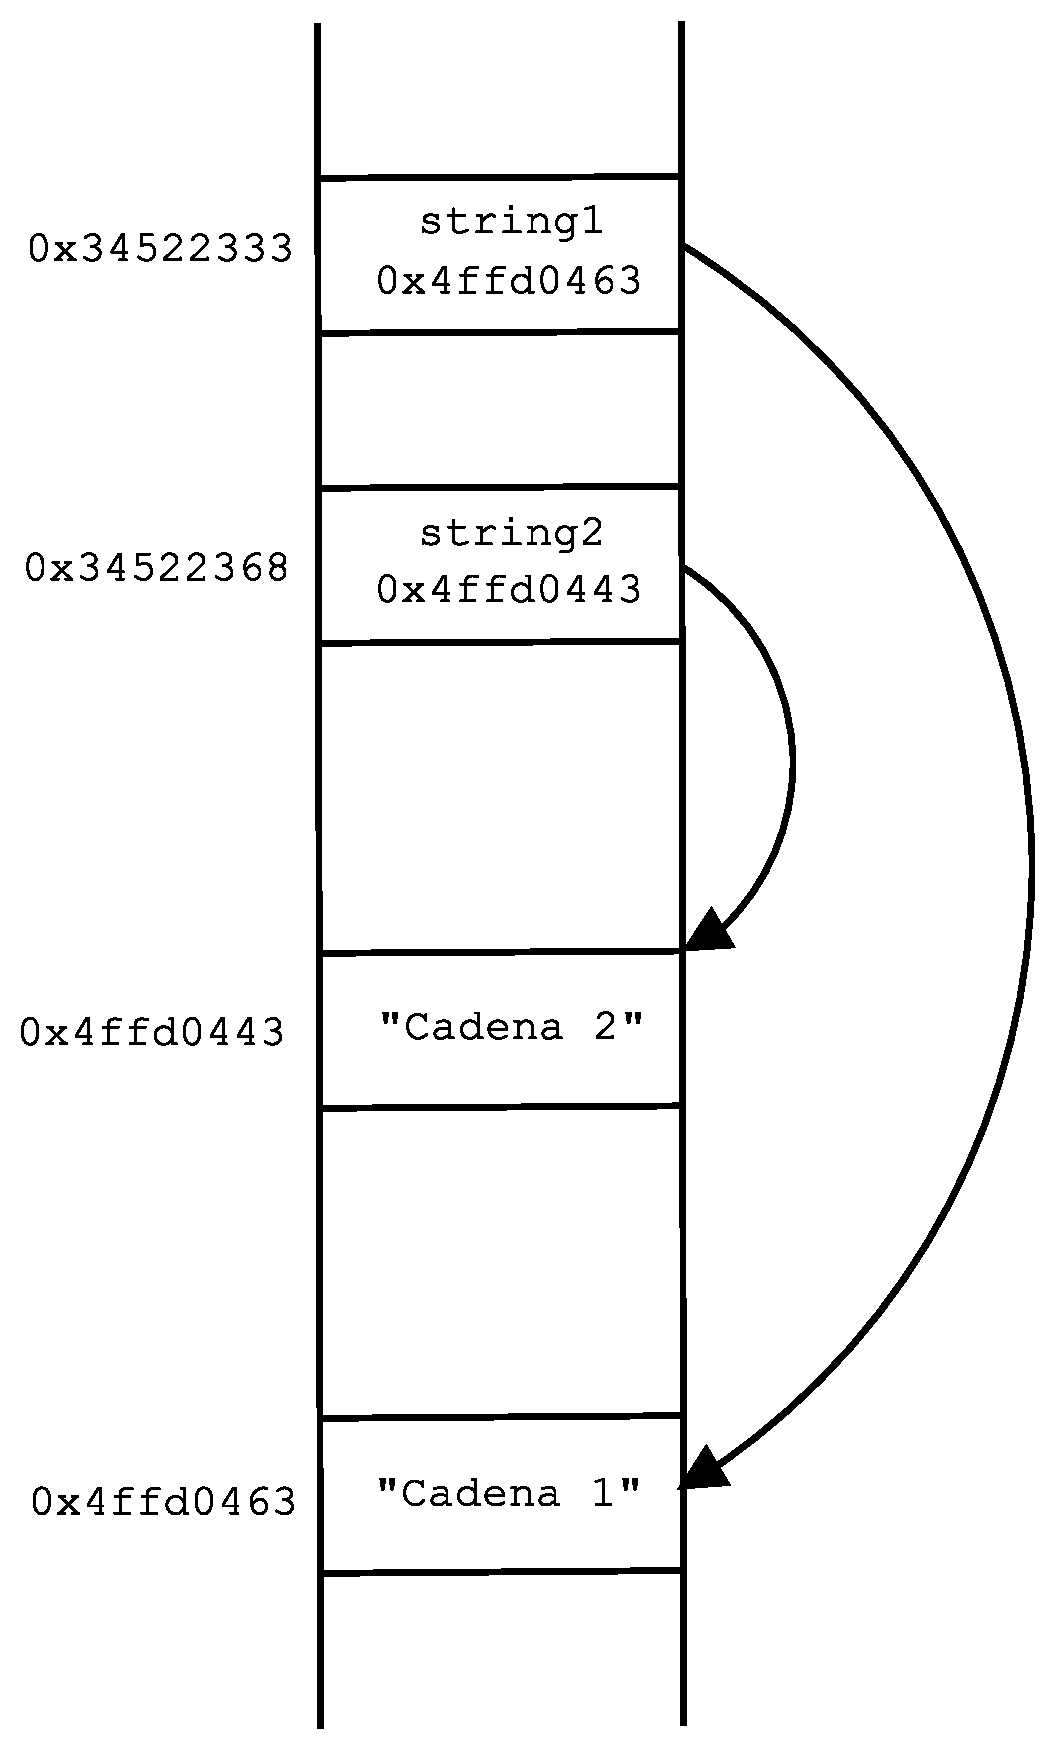
\includegraphics[height=9cm]{punteros/errores/strings.eps}
    \caption{Colocaci�n de strings en memoria}
  \end{center}
\end{figure}

Al observar el diagrama, se entiende m�s facilmente que el c�digo anterior 
no es correcto, esto es, �nicamente compara el valor de las variables
\texttt{string1} y \texttt{string2}, que son las direcciones de memoria
de las cadenas de caracteres, y no las cadenas en s�.\\

Por este motivo, si queremos comparar dos cadenas de caracteres correctamente,
deberemos usar las funciones de la librer�a est�ndar de C que operan sobre strings.
En concreto, la funci�n a utilizar es \texttt{strcmp}\footnote{Explicada m�s
 detalladamente en la secci�n \ref{strcmp}}, que compara dos cadenas 
car�cter a car�cter.\\

De esta manera, el c�digo corregido quedar�a:

\ejemplo{punteros/errores/strings_ok.c}

%%%%%%%%%%%%%%%%%%%%%%%%%%%%%%%%%%%%%%%%%%%%%%%%%%%%%%%%%%%%%%
%
%%%%%%%%%%%%%%%%%%%%%%%%%%%%%%%%%%%%%%%%%%%%%%%%%%%%%%%%%%%%%%

\subsection{Punteros ``a Roma"\ (\textit{memory leaks})}
\label{punteros_roma}

Observemos lo que ocurre en el siguiente ejemplo:
\ejemplo{punteros/errores/roma.c}

Al ejecutar el programa anterior, obtendr�amos el siguiente
diagrama:
\begin{figure}[H]
  \begin{center}
    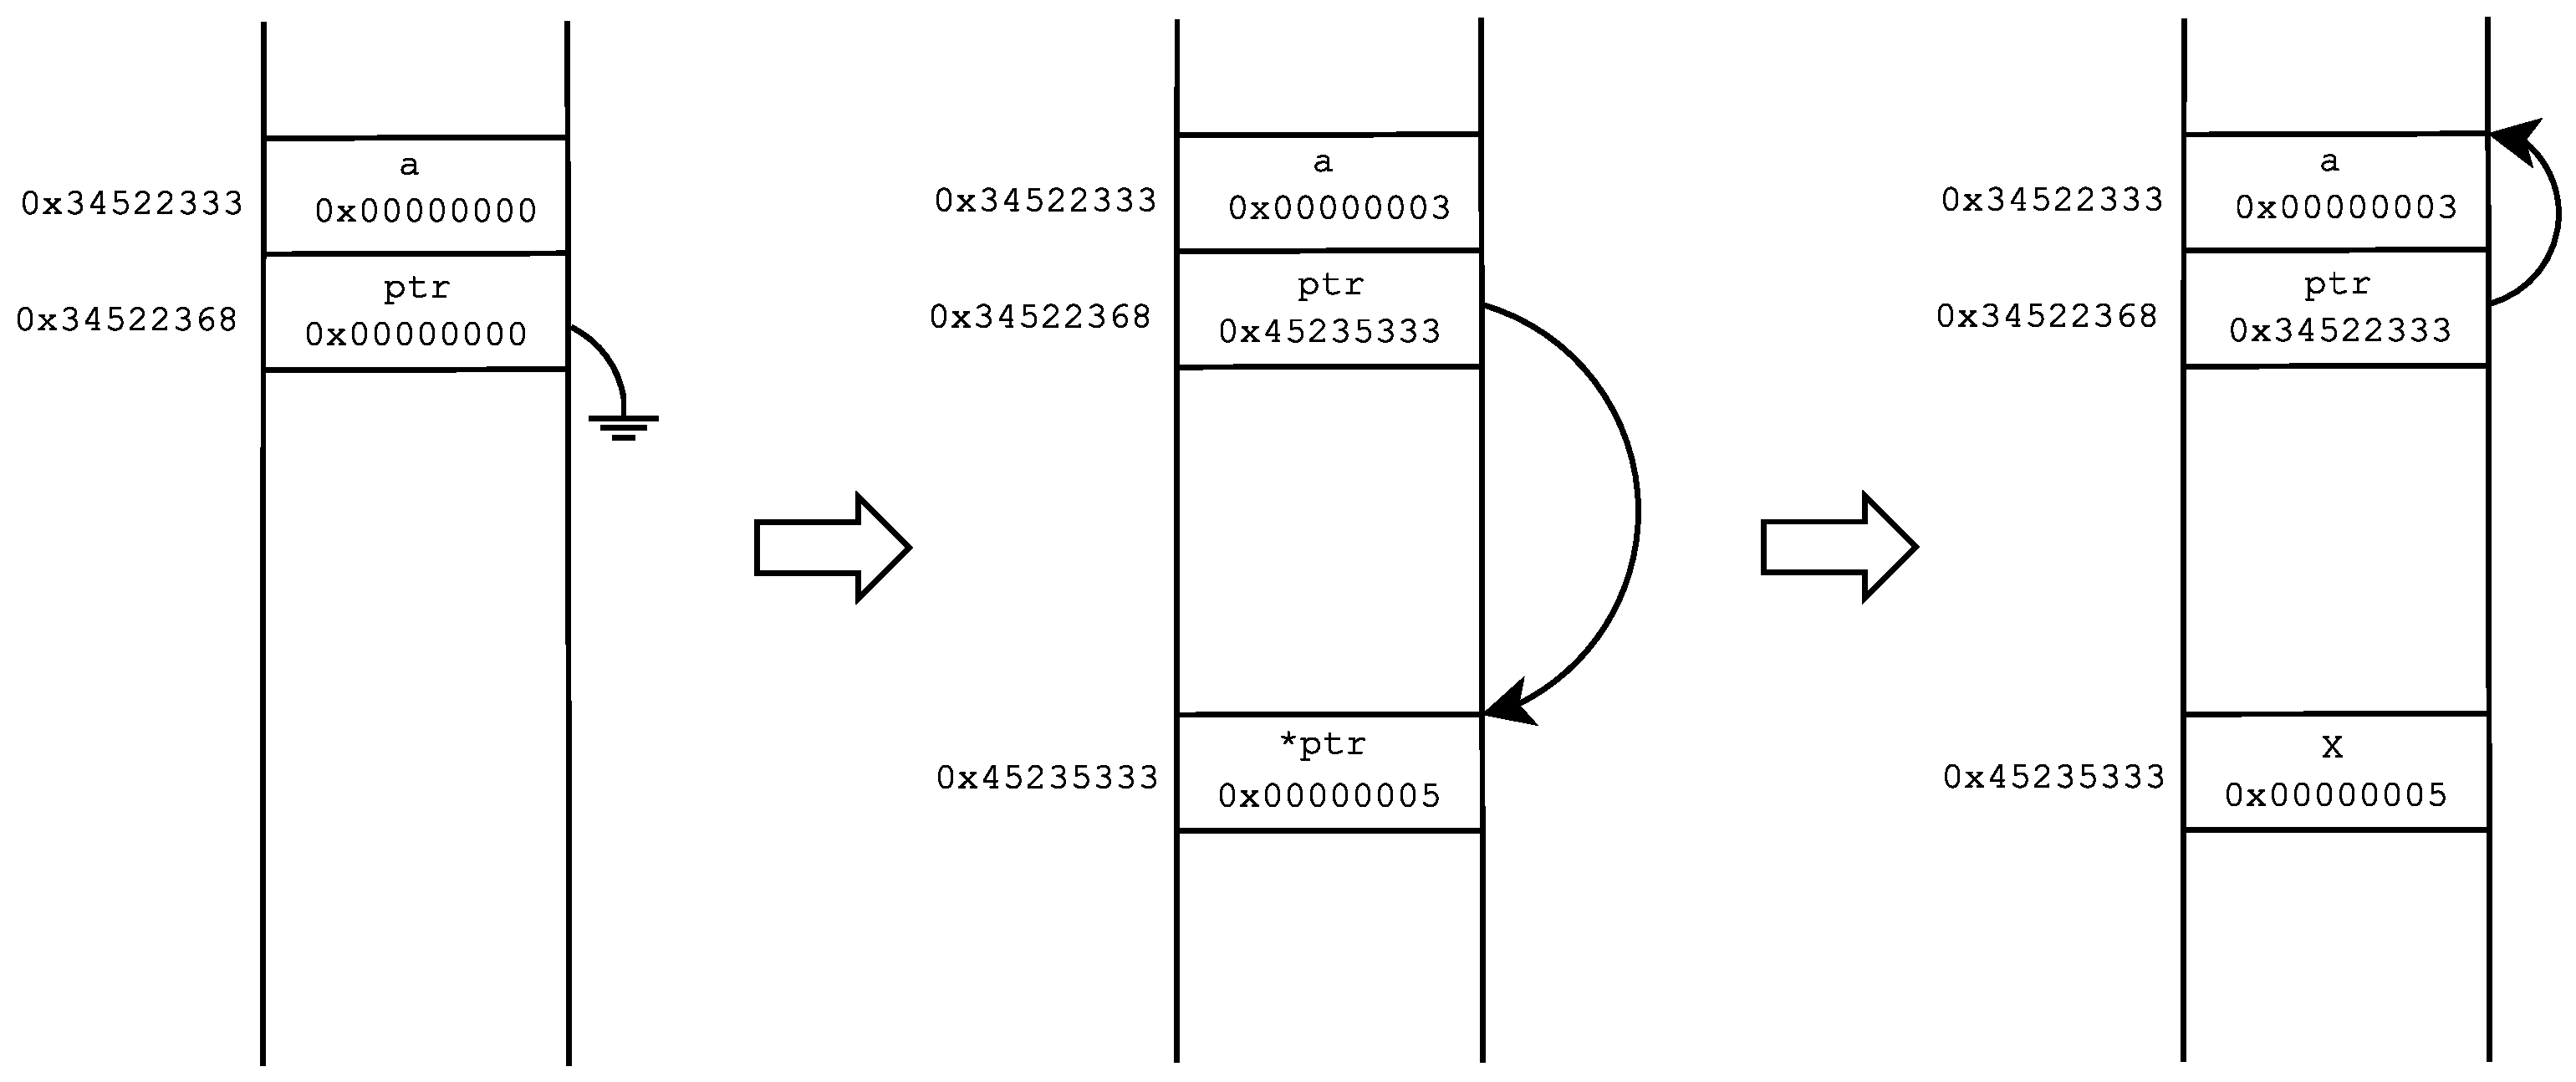
\includegraphics[width=14cm]{punteros/errores/roma.eps}
    \caption{Punteros a roma}
  \end{center}
\end{figure}

Como se puede apreciar, en la finalizaci�n del programa, ha quedado
una zona de memoria (\verb+0x45235333+) ocupada, que no esta apuntada
por ninguna variable. Esto implica no poder acceder al contenido
de dicha zona y por tanto, no poder liberarla, con el consiguiente
gasto innecesario de memoria.
%%%%%%%%%%%%%%%%%%%%%%%%%%%%%%%%%%%%%%%%%%%%%%%%%%%%%%%%%%%%%%
%
%%%%%%%%%%%%%%%%%%%%%%%%%%%%%%%%%%%%%%%%%%%%%%%%%%%%%%%%%%%%%%

\subsection{Doble liberaci�n}
\label{error_doble_liberacion}
Cuando se programa utilizando memoria din�mica, es necesario
liberar toda la memoria solicitada, pero �nicamente 
es necesario realizarlo una vez.
En ocasiones, se intenta liberar varias veces la misma zona de
memoria, consiguiendo un \texttt{Segmentation Fault}, pues
esta memoria ya estaba marcada como libre. Se puede comprobar con
un ejemplo muy simple como el siguiente:
\ejemplo{punteros/errores/mem.c}

%%%%%%%%%%%%%%%%%%%%%%%%%%%%%%%%%%%%%%%%%%%%%%%%%%%%%%%%%%%%%%
%
%%%%%%%%%%%%%%%%%%%%%%%%%%%%%%%%%%%%%%%%%%%%%%%%%%%%%%%%%%%%%%

\subsection{Usar $.$ en lugar de \texttt{->}}
Al utilizar estructuras apuntadas por punteros, hemos de tener
precauci�n y utilizar correctamente los operadores $.$ y \verb+->+
Vemos un mal uso de ellos en el siguiente ejemplo:

\ejemplo{punteros/errores/structs1.c}

%Y como se deber�a utilizar correctamente:
Y cual es su uso correcto:

\ejemplo{punteros/errores/structs2.c}


\label{error_considerar_puntero}


%%%%%%%%%%%%%%%%%%%%%%%%%%%%%%%%%%%%%%%%%%%%%%%%%%%%%%%%%%%%%%
%
%%%%%%%%%%%%%%%%%%%%%%%%%%%%%%%%%%%%%%%%%%%%%%%%%%%%%%%%%%%%%%

\subsection{Operar con los punteros en lugar de con los contenidos}
En los programas que utilizan punteros (memoria din�mica), es imprescindible
diferenciar perfectamente entre el puntero en s� y su contenido,
pues en otro caso, realizaremos algunas operaciones sobre el puntero
cuando en realidad queremos hacerlas sobre el contenido
\footnote{Un caso de este tipo es comentado m�s en detalle en
la secci�n \ref{error_confundir_strings_punteros}}. Veamos algunos errores m�s frecuentes:

\ejemplo{punteros/errores/contenido1.c}

Ahora la versi�n correcta:

\ejemplo{punteros/errores/contenido2.c}



%%%%%%%%%%%%%%%%%%%%%%%%%%%%%%%%%%%%%%%%%%%%%%%%%%%%%%%%%%%%%%
%
%%%%%%%%%%%%%%%%%%%%%%%%%%%%%%%%%%%%%%%%%%%%%%%%%%%%%%%%%%%%%%
\subsection{Finalizaci�n de cadenas}

En el lenguaje C, las cadenas de caracteres deben tener un
car�cter de finalizaci�n, \verb+\0+. Cuando asignamos
o inicializamos una variable con una cadena entre comillas dobles, el 
car�cter de finalizaci�n es puesto autom�ticamente por
el compilador, por ejemplo:

\begin{verbatim}
char * string1 = "Cadena";
\end{verbatim}

El c�digo anterior inicializar� la variable de la siguiente manera:
\begin{figure}[H]
  \begin{center}
    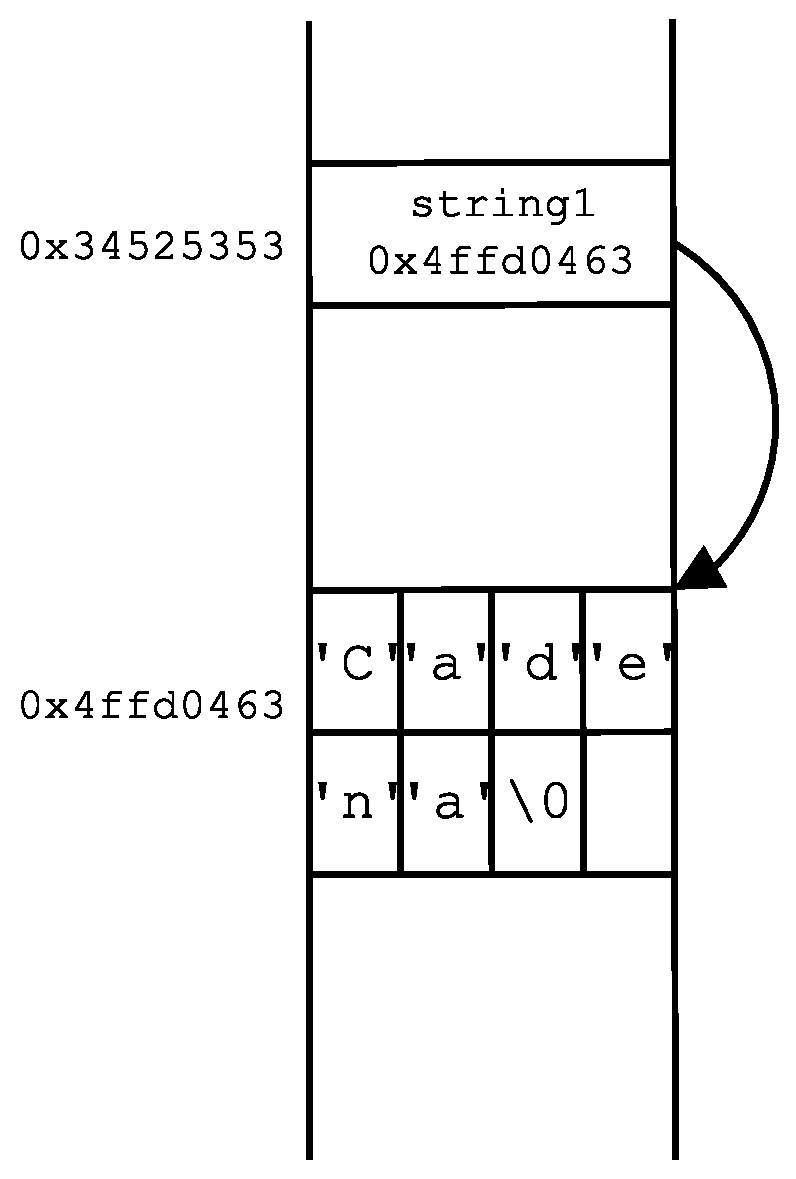
\includegraphics[height=7.5cm]{punteros/errores/cadena.eps}
    \caption{Car�cter de finalizaci�n}
  \end{center}
\end{figure}

De esta forma, en tiempo de ejecuci�n, al operar sobre una cadena
se busca el car�cter \verb+\0+, que indique el fin
de la misma. Es por esto que si se olvida poner dicho indicador 
cuando se est� rellenando una cadena car�cter a car�cter 
(en un bucle, por ejemplo), al intentar acceder a ella,
el programa seguir� leyendo la informaci�n que exista a continuaci�n
de la cadena hasta que muy probablemente intente acceder a una zona
en la que no tenga permisos y termine con el t�pico \texttt{Segmentation
Fault}.


